\chapter{Experiments}
\label{c:experiments} To evaluate different versions of collaborative filtering algorithms and compare their performance to social collaborative filtering algorithms, simulations were run with the help of software designed specifically for this purpose. This chapter explains the experiments that were conducted and explains and interprets the results. The five basic experiments were:

\begin{enumerate}
\item Different versions of user-based collaborative filtering are evaluated on the last.fm dataset.
\item Different versions of social user-based collaborative filtering are evaluated on the last.fm dataset and their performance is compared to the performance of the conventional ones.
\item Different artificially generated networks and ratings are used to again compare collaborative filtering and social collaborative filtering and find conditions under which social collaborative filtering might perform better.
\item The hypothesis that central users in communities might be better predictors was analyzed.
\item The hypothesis that social collaborative filtering works better for certain users was analyzed.
\end{enumerate}

\section{Experimental Setup}
\label{st:experimentalsetup}

\subsection{Last.fm Dataset}
\label{sst:lastfmdataset} The dataset from last.fm is publicly available and can be obtained from the ``Social Computing Research at the University of Minnesota'' website \cite{Grouplens}. It contains information about 1892 (anonymized) users and 17632 artists. Since the users on last.fm do not explicitly give ratings to an artist, the degree to which a user likes or dislikes an artist is expressed as ``listening-count'' (how many times a user has listened to an artist). There are 92'834 $(user, artist, listeningcount)$-tuples. The dataset further contains 12'717 bi-directional user friend relations in the form of $(user_i, user_j)$-pairs. The dataset further also contains informations about tags that users assigned to artists, but these will not be used in the experiments. However, the friend relations will be used and are indeed very important for the social collaborative filtering algorithms.

\subsubsection{Normalization and cleaning-up of the Dataset}
\label{sst:normalizationandcleaningup} The rating file consisting of $(user, artist, listeningcount)$-tuples can already be used as input for a recommender algorithm. With k-fold cross-validation, the tuples can be partitioned into training and test sets. The problem is that the performance of the algorithms will be quite hard to evaulate, since the RMSE that is often used to measure the performance largely depends on the range of the ratings. The listeningcounts that are used as ratings in the last.fm dataset range from 1 to 352'698. There are users who have listeningcounts in the range of a couple of dozen, and others that only have listeningcounts beyond 1'000. This suggests that the listeningcounts need to be normalized so that the resulting RMSE's can acually be interpreted to make statements about the performance of the recommender algorithms.

There are a few steps in the normalization and clean-up process. Firstly, the few users that have the same listeningcount 1 for every artist they have listened to are completely removed. There is no information about the preferences of those users contained in their ratings. It is justifiable to do this since real recommender systems will hardly ever have to deal with a user that gives every item the same rating. Secondly, users with less than 10 ratings are also removed. This is done because of the partitioning of the dataset into training and test sets. There should always be users in both the partitioning and the training set, even if k is as high as 10.

After these removals have been performed, the listeningcounts need to be normalized in the following way:
\newline

\begin{algorithm}[H]
\SetAlgoLined
\KwData{All $(user,artist,listeningcount)$-tuples $x=(u,a,l) \in X$, min (e.g. 1), max (e.g. 5)}
\KwResult{Normalized $(user,artist,rating)$-tuples $x'=(u,a,r) \in X'$ with $r$ between min and max}
\For{$u \in X$}{
currentMin = findMinimum(u)\;
currentMax = findMaximum(u)\;
\For{each $x$ with $x(u)=u$}{
normalizingFactor = $\frac{x(l) - currentMin}{currentMax - currentMin}$\;
r = $normalizingFactor \cdot (max-min) + min$\;
$x'=(u,a,r)$\;
}
}
\caption{Normalize Ratings}
\end{algorithm}

After this algorithm is run, all ratings are in the range $[min,max]$ and are suited as input for the recommender algorithms. As a consequence, the friend relations also need to be updated. All relations containing one of the users removed beforehand are also removed. This leaves us with 92'770 of the original 92'834 ratings and 12'508 of the original 12'717 friend relations.

\subsection{K-fold Cross-Validation}
\label{sst:kfoldcrossvalidation} Cross-validation is a technique used in statistical analysis to evaluate the accuracy of a prediction model on a given dataset. The dataset is partitioned into a training set, which will be used to ``train'' the model or algorithm, and a test set, which will be used to measure the prediction accuracy.

In k-fold cross-validation, the dataset is randomly split into $k$ subsets of equal size. One of the subsets will serve as the test set and the other $k-1$ will be used as the training set. This is repeated $k$ times, with each subset serving as test set exactly once. This method has the advantage over completely random splitting that each data point is guaranteed to be used in the test set (exacty once).
%EXPERIMENT1
\section{Experiment 1}
\label{st:experiment1} The first experiment was run on the normalized last.fm dataset with the goal of comparing the performance of different versions of user-based collaborative filtering algorithms. The dataset was split using 5-fold cross-validation. To adjust the cross-validation to this particular setting, the process was adjusted a little. Instead of randomly partitioning the 92'770 ratings into 5 subsets, this was done for every user's ratings seperately. This extra step was taken to ensure that for every user there is training data as well as test data.

The two different similarity measures and the three prediction measures presented in section \ref{sst:formalframework} were tested in all possible combinations. The neighbourhood sizes were determined either by a fixed number $n$ (from 1 up to all users) or a similarity threshold $\lambda$ was applied (from 0.0 to 1.0). All resulting parameter combinations were applied to the 5-fold cross-validated dataset, and this was done 5 times, resulting in 25 runs for each parameter setting. The resulting RMSE's were averaged over those 25 runs. The results can be seen in figures \ref{f:userbasedn} and \ref{f:userbasedt}.

\begin{figure}[!ht]
\centering
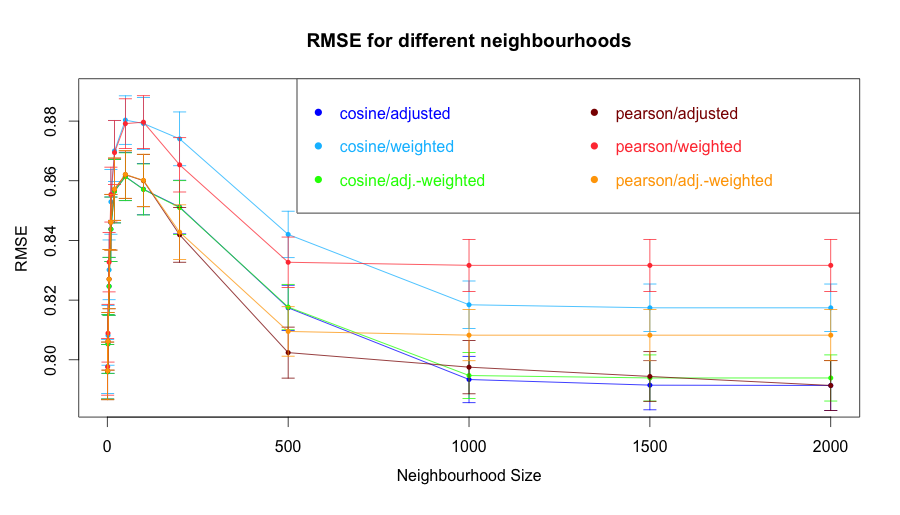
\includegraphics[width=400px]{./4-experiments/figures/USERBASED_N_V4.png}
\caption{Results for neighbourhood}
\label{f:userbasedn}
\end{figure}

\begin{figure}[!ht]
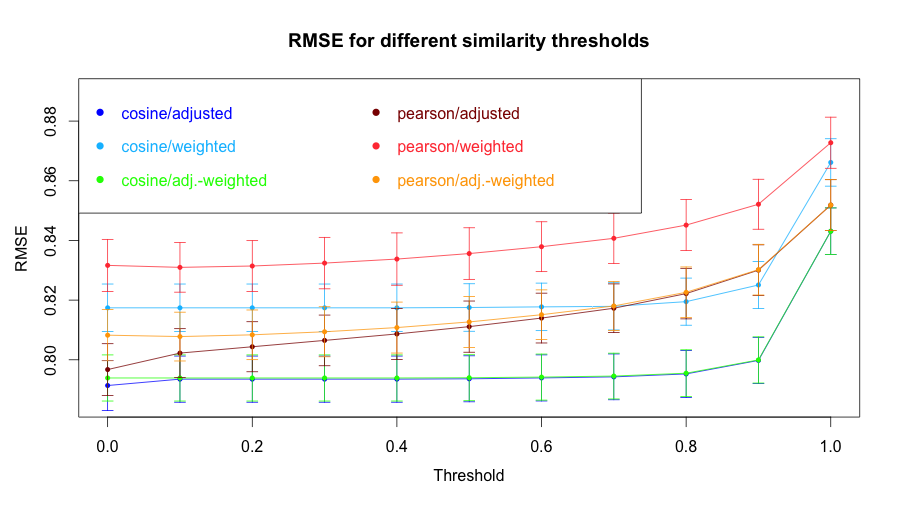
\includegraphics[width=400px]{./4-experiments/figures/USERBASED_T_V4.png}
\caption{Results for threshold}
\label{f:userbasedt}
\end{figure}

It can be seen that the differences between the different similarity measure/prediction measure combinations are relatively small. Averaged over all different neighbourhood options, the combination of cosine similarity and adjusted-weighted sum performs best. Looking at the prediction measures, one can quickly conclude that the consideration of the average rating of a user (as done by the adjusted sum) is more important and makes the predictions more accurate than the consideration of the weights. In fact, the adjusted sum performs almost as good as the adjusted-weighted sum.

Looking at the shapes of all curves, two things stand out: The maximum at neighbourhood $n=50$ and the maximum at threshold $\lambda = 1.0$. At first sight, this is quite astonishing, since other studies have shown a local minimum at neighbourhoods of around 50. It seems weird that there is no such minimum, but instead a clear maximum. To explain these effects, one important realization is to understand that the size $n$ of the neighbourhood $N$ is not necessarily equal to the number of users included in the prediction calculation. As explained in section \ref{sst:formalframework}, out of all users in $N$, only the ones who have actually rated item $j$ can be included in the calculation. In sparse rating matrices, chances are that the actual set of users included in the prediction calculation is much smaller than $n$. For the last.fm dataset with 1'873 users and 17'612 items after normalization, there are 1'873 x 17'612 = 32'987'276 possible ratings of which only 92'770 are actually provided. The rating matrix thus has a density of only 0.3 \% or a sparsity of 99.7 \%. The results suggest that in a setting with very sparse rating matrices, larger neighbourhoods should be chosen so that enough users are included in the prediction.

The dataset of last.fm unveils another characteristic that amplifies this effect: There are many items that have only received one rating. Of course, when the rating for one of these items falls into the test set and has to be predicted, there is no possible information from other users' ratings to take into account. In this case, the algorithm chooses as prediction just the average rating of user $i$ over all his ratings. The experiments showed that the average had to serve as prediction in ${}^1/_2$ of the predictions for a fixed neighbourhood of size 70 (with an average of only 1.87 users per prediction that had actually rated the item). The average of users actually included in the prediction hit 50 at $n = 1050$.

The smaller actual neighbourhood sizes explain why the algorithm gets better with very large neighbourhoods, but they cannot be responsible for the good performance with very small neighbourhoods. The answer for the good performance of the algorithm with neighbourhoods < 10 lies in the performance of the average approach. This approach just returns a user's average over all his ratings as a prediction, and it actually performs pretty well on this dataset. The average RMSE over 5 5-fold cross-validations was 0.78. With very small neighbourhoods, a lot of averages have to be used, which makes the predictions better.

In the case of a similarity threshold, the explanation has to be found elsewhere. There, the actual neighbourhoods often have a decent size. The problem of a similarity threshold of 1.0 is that only users whose ratings are perfectly correlated are included in the prediction. This is, with very few exceptions, only the case if the users have co-rated only one item and given it the same rating. Of course, the similarity of those users results to 1.0, but with only one co-rated item the meaningfulness of this number can be questioned. With a similarity threshold of 1.0, consequently a lot of the users in the neighbourhood are not necessarily very similar to user $i$, which explains the large RMSE for all prediction and similarity measures. In the experiments, the average number of co-rated items for threshold 1.0 was 1.00 while for threshold 0.9 it was 3.10.
%EXPERIMENT2
\section{Experiment 2}
\label{st:experiment2} The second experiment was conducted to measure the influence of the inclusion of social network information on the performance of collaborative filtering. For this, different versions of social collaborative filtering were implemented and tested on the same dataset that was also used for experiment 1. As prediction measure, the adjusted-weighted sum was used and the similarities between users were calculated with the cosine similarity coefficient.

As explained in section \ref{sst:socialcf}, the main difference of social collaborative filtering in comparison to the conventional approach is the choice of the neighbourhood set $N$. Instead of using either a fixed size of the most similar users or applying a threshold, the users closest to user $i$ in the social network can be chosen as his neighbourhood. In this experiment, the friend graph of every user was traversed with a breadth-first search (BFS), and different levels of the resulting node tree were taken as neighbourhoods. If all nodes with distance 1 are included, this corresponds to all direct friends of a user. Distance 2 corresponds to the user's friends and all their friends, and so on.

\begin{figure}[!ht]
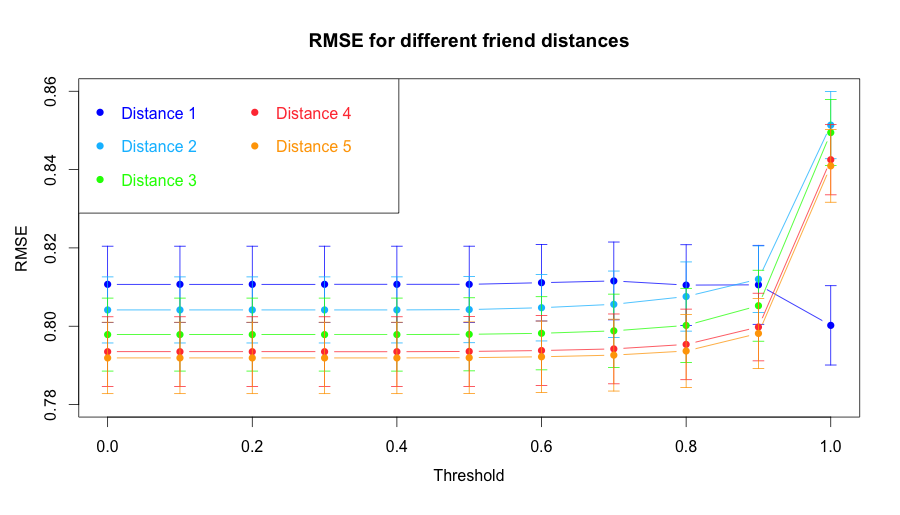
\includegraphics[width=400px]{./4-experiments/figures/SOCIALUSERBASED_V3.png}
\label{f:socialuserbased}
\caption{Results for social collaborative filtering}
\end{figure}

The results seen in figure \ref{f:socialuserbased} show some interesting behaviour. The case where only a user's direct friends are included in the neighbourhood set (\textit{Distance 1}) shows slightly different behaviour than the others. While all other algorithms show a significant drop in performance with a similarity threshold of 1.0, the \textit{Distance 1}-algorithm performs best at this threshold. The explanation for this behaviour can also be found in the fact that with small neighbourhoods and large thresholds, the user's average must be used for a lot of predictions, because there are no users in the neighbourhood who have rated the item to predict. Since the average algorithm (see experiment 1, section \ref{st:experiment1}) actually also performs better than the social user-based CF algorithms, this makes the \textit{Distance 1}-algorithm better at threshold 1.0.

The other algorithms with larger distances consequently have larger neighbourhood sets. Due to this, their behaviour is very similar to the conventional CF algorithms, which also show a performance drop at threshold 1.0. The explanation for this is given in section \ref{experiment 1}.
\newline

Another factor that needs to be considered is the runtime of the algorithms. While in the conventional CF, this factor did not play a big role and all algorithms had similar runtimes, the social CF algorithms show significant differences.

\begin{table}[h]
	\begin{center}
	\begin{tabular}{ | c | c | c |}
	\hline
	Algorithm & mean RMSE & mean runtime (s) \\ \hline
	Distance 1 & 0.810 & 0.25 \\ \hline
	Distance 2 & 0.810 & 2.19 \\ \hline
	Distance 3 & 0.804 & 28.16 \\ \hline
	Distance 4 & 0.799 & 96.28 \\ \hline
	Distance 5 & 0.797 & 127.66 \\ \hline
	\end{tabular}
	\caption{RMSE and runtime of all social CF algorithms}
	\label{t:rmseruntimesocialcf}
	\end{center}
\end{table}

Table \ref{t:rmseruntimesocialcf} shows the mean RMSE and the mean runtime of the social CF algorithms over all runs. While the gain in performance with larger friend distances is marginal, the time for the computation of the neighbourhood set increases significantly. This is largely due to the breadth-first search-like traversing of the friend graph, that takes a lot of time with increasing distances.

These results suggest that the benefit gained from including friends with distance 3 or more does not outweigh the loss in performance. Since the results very much resemble those from conventional CF, it can even be assumed that the inclusion of information from the social network does not improve performance for this specific dataset from last.fm at all. If this were the case, we would expect the algorithms who include socially close users (distances 1 or 2) to perform better.
%EXPERIMENT3
\section{Experiment 3}
\label{st:experiment3} After experiments 1 and 2 which were both run on the same dataset from last.fm, experiment 3 was run to compare the performance of CF and social CF in different environments. For this, instead of real-world data, artificially generated data was used. With a social network generated by the algorithm described in section \ref{st:artificialnetworkgeneration}, rating datasets were generated with different parameters. The parameters used are described in table \ref{t:ratinggenerationparameters}.

\begin{table}[h]
	\begin{center}
    	\begin{tabular}{ | l | l | l | p{5.5cm} |}
   	 \hline
    	Parameter & Variable & Values & Explanation \\ \hline
    	Size of community item set & q & 50, 100, 200, 400 & This is the size of the item set that each community has. It is included in the rating generation so that users of the same community have a higher probability of rating the same items.  \\ \hline
    	Probability of community set & p & 0.05, $^1 / _3$, $^2 / _3$, 1 & This is the probability that for a user's rating, the item is chosen from the whole item set. 1 - p is the probability that it is chosen from the user's community's item set. \\ \hline
    	Influence of item quality & a & 0, $^1 / _3$, $^2 / _3$, 1 & This is a factor in the range [0,1] that determines the influence of the item quality in the rating generation \\ \hline
    	Influence of user taste & b & 0, $^1 / _3$, $^2 / _3$, 1 & This is a factor in the range [0,1] that determines the influence of the user taste in the rating generation \\ \hline
    	Influence of community taste & c & 0, $^1 / _3$, $^2 / _3$, 1 & This is a factor in the range [0,1] that determines the influence of the community taste in the rating generation \\ \hline
    	\end{tabular}
    	\caption{Rating generation parameters}
    	\label{t:ratinggenerationparameters}
    	\end{center}
\end{table}

The rating generation algorithm was run with all these parameter combinations, with the restriction that $a+b+c=1$. This resulted in 160 test runs. For all runs, the same generated social network was used, to prevent any random differences in the results that could have been caused by the network generation.

Every generated rating set was partitioned using 5-fold cross-validation and both conventional and social CF algorithms were run on it. Conventional CF was run with different similarity thresholds and social CF was run with neighbourhood sets consisting of direct friends and friends of friends (distances 1 and 2), also with different similarity thresholds applied.
\newline

The results are interesting and complex. It would be tedious to explain the outcome of every parameter combination in detail, but rather some clear tendencies and dependencies are highlighted.

\begin{itemize}
\item It is clear that the average size of the neighbourhood is largest with the conventional approach, since it includes all users before applying a similarity threshold. The \textit{distance 2}-algorithm uses smaller neighbourhoods, while the \textit{distance 1}-algorithm results in the smallest neighbourhoods. As a consequence, in settings where community taste has little or no influence (c is low), conventional CF performs best, followed by distance 2 social CF and distance 1 social CF. With only your friends in the neighbourhood, the actual set of users included in the prediction is too small to make good predictions (since there is no large correlation between friends). As an example see figure \ref{f:result01}. In this case, the item quality accounts for $^2 / _3$ of the generated rating and the user's individual taste for the other $^1 / _3$. Since item quality is an important factor, the inclusion of more users who have also rated the item will make the prediction better. The massive drop in performance at threshold 1.0 can be explained again by the shrinking of the neighbourhood set and thus the smaller number of users actually included in the prediction.
\item When the community taste has a lot of influence on the performance (c is large), we should expect social CF to perform better in comparison to conventional CF. This is indeed the case, as can be seen in figure \ref{f:result02}. They direct friends of a user are likely to be in the same community and since the community taste has a big influence, those users are better predictors than other users in the network. The significant drop at threshold 1.0 is again due to the neighbourhoods getting really small, with the consequence of having a lot of prediction made by taking users' average ratings. The average-based algorithm performs worse than the CF algorithms in this setting (with a mean RMSE of 0.762), as opposed to the last.fm dataset where it showed better performance than the CF algorithms.
\item All the algorithms show special behaviour at similarity threshold 1.0. This threshold implies that users whose ratings perfectly correlate with a user's ratings should be included in the prediction. Doing this does not make that much sense in most environments. Requiring perfect correlation will in many cases mean to leave out very similar users who might have co-rated a large set of items and only show minor differences in rating behaviour. But one differing rating is enough to make the similarity drop below the threshold of 1.0. The problem is therefore that in most environments, users only have similarity 1.0 if they have only co-rated a small number of items (most often 1 item) and those ratings are the same.
\end{itemize}

\begin{figure}[!h]
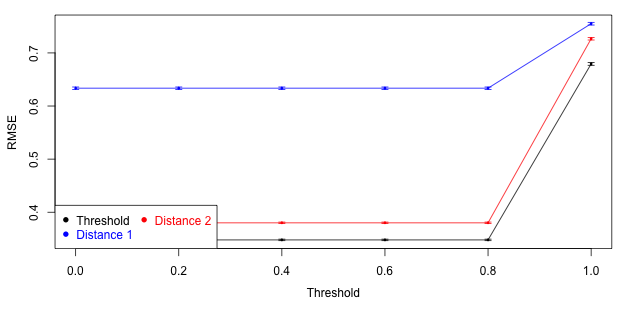
\includegraphics[width=400px]{./4-experiments/figures/Result2_50_066_033_033.png}
\caption{RMSE's for parameters q = 50, p = $^1 / _3$, a = $^2 / _3$, b = $^1 / _3$, c = 0}
\label{f:result01}
\end{figure}

\begin{figure}[!h]
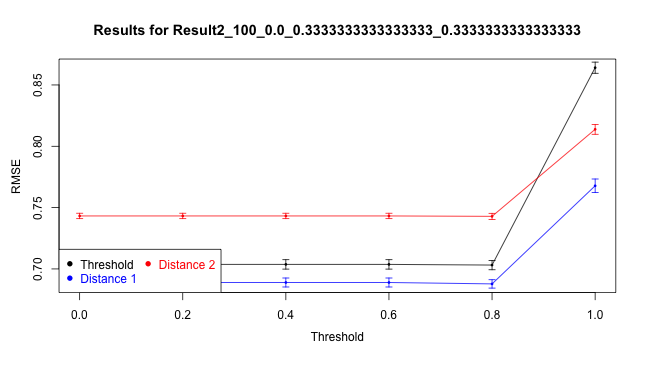
\includegraphics[width=400px]{./4-experiments/figures/Result2_100_00_033_033.png}
\caption{RMSE's for parameters q = 100, p = $^1 / _3$, a = 0, b = $^1 / _3$, c = $^2 / _3$}
\label{f:result02}
\end{figure}
%EXPERIMENT4
\section{Experiment 4}
\label{st:experiment4} Experiment 4 aimed to analyze if users that are central in a social network or in a community within the network could be better predictors than others. This hypothesis was tested on the last.fm dataset. Using the similarities between users, it was tested if there was a stronger correlation of users with central and influential people than with the rest of a community.
\newline

The experiment was conducted in the following way:

\begin{enumerate}
\item A community detection algorithm was run on the last.fm social network and every user was put into one community. As community detection algorithm (see section \ref{sst:communityalgorithms}), for this experiment the walktrap algorithm of \cite{Pons_2005} was chosen since it seems to partition the network into more and smaller communities than the modularity optimization algorithm by \cite{Clauset_2004}, which suffers a resolution limit (see \cite{Fortunato_2007}) and would partition the network into only few communities that are very large.
\item The users are sorted by decreasing centrality. As centrality measure, betweenness centrality is chosen (see \ref{sst:graphproperties}).
\item For each community, the $n$ most central users are put into a group of \textit{influencers}.
\item For each user, the average rating similarity between him and the \textit{influencers} is calculated.
\item Steps 3 and 4 are repeated for all $n$ from 1 to 100.
\item Additionally, the average rating similarity between users and their community is calcuated for each user, and then averaged.
\end{enumerate}

The resulting similarities can be seen in figure \ref{f:influencersimilarity}. The red line is the average correlation of users with their community calculated in step 6. The blue dots indicate the similarities with the group of \textit{influencers} calculated in steps 3 and 4, for $n$ between 1 and 100. It is clear that the blue line will converge to the red line, since for very large $n$'s the \textit{influencer} group will consist of the whole community and thus be equal to the red line.

\begin{figure}[!h]
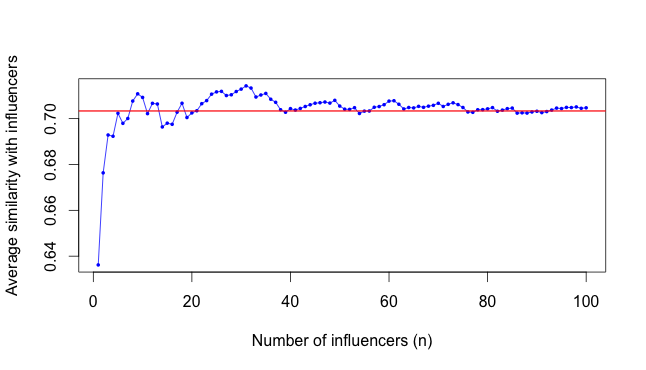
\includegraphics[width=400px]{./4-experiments/figures/InfluencerSimilarities_2.png}
\caption{Average similarity of users with \textit{influencers}}
\label{f:influencersimilarity}
\end{figure}

These results are a clear indication that some users in communities have influence on the taste (and therefore on the rating behaviour) of other users in those communities. At $n=31$, the maximal similarity of 0.715 can be found, which is above the average rating similarity between users and their whole community (0.703). With this insight, one could possibly improve the social CF algorithm by taking into account information about centrality (e.g. by giving central users more weight in the prediction).
%EXPERIMENT5
\section{Experiment 5}
\label{st:experiment5} The last experiment aimed to answer the question if there are users or groups of users for which social CF works better. After experiment 4 (section \ref{st:experiment4}) showed that there exist users that are better predictors than others because of their position and influence in the social network, the next question to ask is whether there are also positions in the network or factors that influence how well social CF performs for specific users in those positions.
\newline

To examine this question, the last.fm dataset was once again studied. The set was partitioned with 5-fold cross-validation and then conventional CF algorithms were run as well as social CF algorithms, each with different similarity thresholds from 0.0 to 1.0. Instead of calculating the average RMSE for a whole run as in previous experiments, RMSE's were collected for each user individually. Then, for each user, averages were taken over all conventional CF runs and over all social CF runs. The average social CF RMSE was subtracted from the average conventional CF RMSE for each user. Negative results imply that conventional CF works better for that user, while positive results imply that social CF works better. This error difference was stored for each user and users were sorted by their error difference, in ascending order. The result can be seen in figure \ref{f:usererrors}.

\begin{figure}[!h]
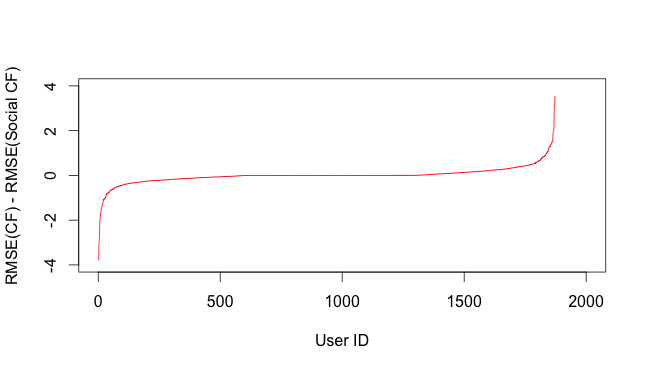
\includegraphics[width=400px]{./4-experiments/figures/UserErrors.png}
\caption{Average conventional CF RMSE - average social CF RMSE of all users, sorted from lowest to highest}
\label{f:usererrors}
\end{figure}

Figure \ref{f:usererrors} shows that with very few exceptions, the difference between CF and social CF RMSE's lies between -0.5 and 0.5. There are only 15 users with a difference $<$ -0.5 (the ones at the very left in figure \ref{f:usererrors}), and only 13 users with a difference $>$ 0.5 (the ones at the very right). The assumption that social CF might work better for users with many friends (central users) does not prove to be true, as there are central as well as decentral users on both ends of the scale.

The RMSE differences are quite small overall, revealing no specific group of users for which social CF seems to work better than conventional CF. However, it is clear that in many settings, social CF will indeed work better for users that are in a community that influences the taste of its members.
%DISCUSSION
\section{Discussion}
\label{st:discussion} The experiments that were conducted showed the behaviour of CF and social CF in different situations and settings. The most important and interesting take-aways will be discussed in this section.
\newline

First, it appears that the cosine similarity measure performs slightly better than the pearson correlation similarity measure. Although both measures are very similar, the algorithms using cosine similarity perform a bit better, except in situations with very small neighbourhoods. However, the differences are not very large and the general behaviour of both measure seems to be the same. \cite{Lathia_2008} even stated that in their analysis of similarity measures, using a random similarity measure sometimes yielded better results than using one of the popular approaches (also see \cite{Amatriain_2011}).

Comparing the different prediction measures, the experiments suggest that the weighing of the ratings with the users' similarities does not affect the prediction as much as adjusting it to the average ratings. Using the adjusted sum yields almost the same results as using the adjusted-weighted sum, while using only the weighted sum results in worse performance.

A very important point to consider when using neighbourhood-based algorithms is the sparsity of the rating matrix. As already highlighted in experiment 1, a sparse rating matrix can lead to the effect of actually having very few users included in the prediction calculation, which worsens the performance of CF and social CF algorithms. This problem is known as new-user or new-item problem (also see section \ref{ssst:challengescf}), and it is a known challenge of the CF approach to make predictions in environments with very sparse rating matrices.

\begin{figure}[!h]
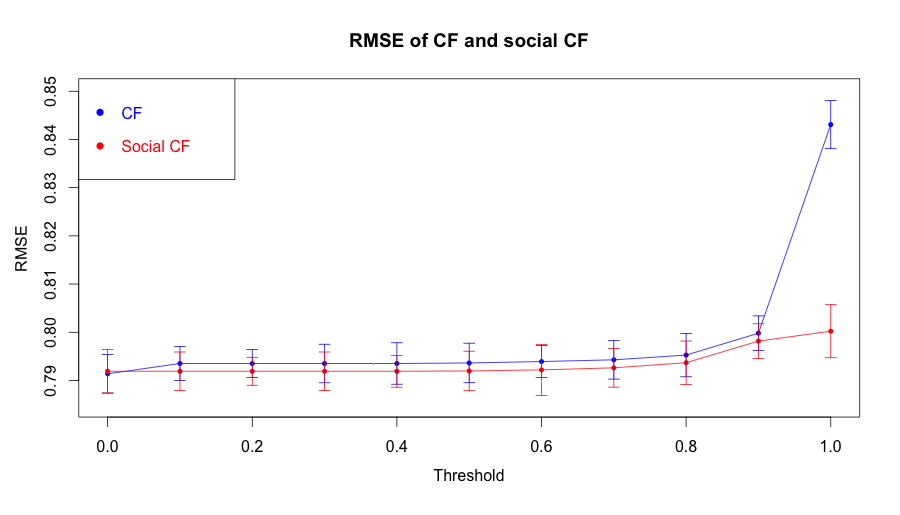
\includegraphics[width=400px]{./4-experiments/figures/CFvsSocialCF_01.png}
\caption{Best CF vs best social CF performances}
\label{f:cfvssocialcf}
\end{figure}

Comparing conventional and social CF directly shows that both approaches work similarly well on the last.fm dataset. Figure \ref{f:cfvssocialcf} shows for both CF and social CF their best algorithm at each threshold, resulting in a (purely theoretical) mixed algorithm that chooses at each threshold the algorithm with the settings that performs best. The social CF algorithms have the edge at every threshold, with the largest difference at threshold 1.0. This is due to the performance of the \textit{Distance 1}-algorithm, which actually gets better at threshold 1.0 (see section \ref{st:experiment2}).
\newline

Experiment 3 showed that the use of social CF can enhance performance in settings where community taste has a stronger influence (see section \ref{st:experiment3}). Although this experiment was performed on artificially generated datasets, the network and rating generation algorithms produce data similar to real-world datasets, and therefore the results strongly indicate that the algorithms would behave similarly in certain real-world settings.
\newline

The last two experiments analyzed the positions of certain users in the network, showing that central users might indeed be better predictors than others. The existence of a rating correlation between users and the \textit{influencers} of their community will have to be further analyzed on other real-world data. The last.fm dataset already revealed this correlation, but there are certainly recommender systems where the social network has more importance than in this specific music streaming environment (e.g. holiday recommendations).